%------------------------------------------------------------------------%
% ABNTEX2: Modelo de Trabalho Acadêmico (tese de doutorado, dissertação de mestrado e trabalhos monográficos em geral) em conformidade com ABNT NBR 14724:2011
% Adaptado por Samuel da Silva Feitosa (2021-02-18) baseado no modelo "Template para elaboração de trabalho acadêmico" disponível na página de documentos úteis do IFSC
%------------------------------------------------------------------------%

\documentclass[
	% -- opções da classe memoir -- %
	10pt,			 	  % tamanho da fonte
	%openright,			  % capítulos começam em página ímpar (insere página vazia caso preciso)
	%twoside,			  % para impressão em frente e verso, ou seja, oposto a oneside
	oneside,
	a4paper,			  % tamanho do papel. 
	% -- opções da classe abntex2 -- %
	chapter=TITLE,		  % títulos de capítulos convertidos em letras maiúsculas
	%section=TITLE,		  % títulos de seções convertidos em letras maiúsculas
	%subsection=TITLE,	  % títulos de subseções convertidos em letras maiúsculas
	%subsubsection=TITLE, % títulos de subsubseções convertidos em letras maiúsculas
	% -- opções do pacote babel -- %
	english,			 % idioma adicional para hifenização
%	french,				 % idioma adicional para hifenização
%	spanish,			 % idioma adicional para hifenização
	brazil				 % o último idioma é o principal do documento
	]{abntex2}

% Todas as indicações de pacotes e configurações estão no arquivo de estilo chamado estilo-monografia-ifsc.sty.
\usepackage{style}	
	
%---------------------------------------------------------------------%
% Informações de dados para Capa e Folha de Rosto
%---------------------------------------------------------------------%

\titulo{APLICANDO DEEP LEARNING EM EXAMES LABORATORIAIS DE SANGUE \\ Desenvolvimento de Laudos e Hemogramas}
\autor{Anthony Cruz}
\local{Caçador - SC}
\data{18 de Junho de 2021}
\orientador{Professor Samuel da Silva Feitosa}
\coorientador{Professor Cristiano Mesquita Garcia}
\instituicao{%
  Instituto Federal de Santa Catarina -- IFSC
  \par
  Campus Caçador
  \par
  Sistemas de Informação}
\tipotrabalho{Monografia (Graduação)}

% O preambulo deve conter o tipo do trabalho, o objetivo, o nome da instituição e a área de concentração
\preambulo{Projeto de Pesquisa apresentado à Coordenadoria do Curso de Sistemas de Informação do Câmpus Caçador do Instituto Federal de Santa Catarina para a avaliar a possibilidade de continuidade do Trabalho de Conclusão de Curso.}
%---------------------------------------------------------------------%

\textoaprovacao{Este projeto foi julgado adequado para continuidade do Trabalho de Conclusão do Curso de Sistemas de Informação, pelo Instituto Federal de Educação, Ciência e Tecnologia de Santa Catarina, e aprovado na sua forma final pela comissão avaliadora abaixo indicada.}


%---------------------------------------------------------------------%
% Início do Documento
%---------------------------------------------------------------------%
\begin{document}
% Seleciona o idioma do documento (conforme pacotes do babel)
\selectlanguage{brazil}
% Retira espaço extra obsoleto entre as frases.
\frenchspacing 

% ----------------------------------------------------------
% Elementos Pré-Textuais
% ----------------------------------------------------------
% \pretextual
\imprimircapa

% Folha de Rosto - (o * indica que haverá a ficha bibliográfica)
\imprimirfolhaderosto
%---------------------------------------------------------------------%

% Folha de aprovação

% Isto é um exemplo de Folha de aprovação, elemento obrigatório da NBR 14724/2011 (seção 4.2.1.3). Você pode utilizar este modelo até a aprovação do trabalho. 
% Após isso, substitua todo o conteúdo deste arquivo por uma imagem da página assinada pela banca com o comando abaixo:%
% \includepdf{folhadeaprovacao_final.pdf}

\begin{folhadeaprovacao}
	\begin{center}
		{\ABNTEXchapterfont\large\MakeUppercase{\imprimirautor}}
		\vspace*{\fill}\vspace*{\fill}
		\begin{center}
			\ABNTEXchapterfont\Large\MakeUppercase{\imprimirtitulo}
		\end{center}
		\vspace*{\fill}
		\imprimirtextoaprovacao
		\vspace*{1cm}
		\imprimirlocal, 18 de junho de 2021.
		\vspace*{\fill}
	\end{center}
		   
	\assinatura{\textbf{\imprimirorientador, Dr.} \\ Orientador\\Instituto Federal de Santa Catarina} 
	\assinatura{\textbf{\imprimircoorientador, Me.} \\ Coorientador\\Instituto Federal de Santa Catarina }
	\assinatura{\textbf{Professor Vitor Sales Dias da Rosa, Dr.} \\ Banca Avaliadora\\Instituto Federal de Santa Catarina}
	\assinatura{\textbf{Professor Fabrício Herpich, Dr.} \\ Banca Avaliadora\\Instituto Federal de Santa Catarina}
	%\assinatura{\textbf{Professor} \\ Convidado 4}
	\vspace*{1cm}  
		  
\end{folhadeaprovacao}

%---------------------------------------------------------------------%
% Resumos
%---------------------------------------------------------------------%
% Resumo em português
\setlength{\absparsep}{18pt} % ajusta o espaçamento dos parágrafos do resumo
\begin{resumo}
	Os exames laboratoriais de sangue, principalmente quando se trata de hemogramas, são um dos tipos de exames mais importantes e mais realizados no âmbito médico. Através dessa prática pode-se descobrir importantes alterações no organismo e é geralmente utilizado como primeiro passo na avaliação da saúde dos pacientes. Embora seja uma prática bastante comum, a sua realização é bastante dificultada nos laboratórios por utilizar um maquinário de alto custo de compra e manutenção. Como alternativa a isso, este projeto tem como objetivo desenvolver um modelo de \emph{Deep Learning} para realizar esse processo utilizando menos recursos, através da interpretação automática de imagens de amostras de sangue em placas de Petri, para assim, ser capaz de elaborar hemogramas de forma automatizada. A partir da elaboração de um mapeamento sistemático da literatura foi possível identificar as principais abordagens de \emph{Deep Learning} (\emph{Convolutional Neural Network} e \emph{Recurrent Neural Network}) que podem ser utilizadas para a resolução do problema abordado.
	
	\textbf{Palavras-chave:} Hemograma. Exames de Sangue. \emph{Deep Learning}. Redes Neurais.
\end{resumo}

% Resumo em inglês
\begin{resumo}[Abstract]
	\begin{otherlanguage*}{english}
		Laboratory blood tests, especially when it comes to Complete Blood Count (CBC), are one of the most important types of tests performed in the medical field. Through this practice, important changes in the body can be discovered, and it is generally used as a first step in the assessment of patients health. Although it is a very common practice, its realization is very difficult in laboratories because it uses machinery with a high purchase and maintenance cost. As an alternative to this, this project intends to develop a Deep Learning model to perform this process using fewer resources, through the automatic interpretation of images of blood samples in Petri dishes, in order to be able to elaborate automated blood counts. From the elaboration of a systematic literature mapping, it was possible to identify the main Deep Learning approaches (Convolutional Neural Network and Recurrent Neural Network) that can be used to solve the problem addressed.
		\vspace{\onelineskip}
		\noindent 
		
		\textbf{Keywords}: Complete Blood Count. Blood Test. Deep Learning. Neural Networks.
	\end{otherlanguage*}
\end{resumo}

%---------------------------------------------------------------------%
% Inserir lista de ilustrações, tabelas, listagem de códigos, abreviaturas, símbolos
%---------------------------------------------------------------------%
\pdfbookmark[0]{\listfigurename}{lof}
\listoffigures*
\cleardoublepage
% inserir lista de tabelas
\pdfbookmark[0]{\listtablename}{lot}
\listoftables*
\cleardoublepage

%---------------------------------------------------------------------%
% Inserir lista de listings (códigos-fonte)
%---------------------------------------------------------------------%
%\pdfbookmark[0]{\lstlistlistingname}{lol}
%\begin{KeepFromToc}
%\lstlistoflistings
%\end{KeepFromToc}
%\cleardoublepage

%---------------------------------------------------------------------%
% Inserir lista de abreviaturas e siglas
%---------------------------------------------------------------------%
\pdfbookmark[0]{Lista de abreviaturas e siglas}{loa}
% Como usar o pacote acronym
% \ac{acronimo} -- Na primeira vez que for citado o acronimo, o nome completo irá aparecer
%                  seguido do acronimo entre parênteses. Na próxima vez somente o acronimo
%                  irá aparecer. Se usou a opção footnote no pacote, então o nome por extenso
%                  irá aparecer aparecer no rodapé.
%
% \acf{acronimo} -- Para aparecer com nome completo + acronimo.
% \acs{acronimo} -- Para aparecer somente o acronimo.
% \acl{acronimo} -- Nome por extenso somente, sem o acronimo.
% \acp{acronimo} -- Igual o \ac mas deixando no plural com S (inglês).
% \acfp{acronimo}--
% \acsp{acronimo}--
% \aclp{acronimo}--

\chapter*{Lista de abreviaturas e siglas}%
% \addcontentsline{toc}{chapter}{Lista de abreviaturas e siglas}
\markboth{Lista de abreviaturas e siglas}{}

\begin{acronym}
    \acro{RBC}{Red Blood Cells}
    \acro{WBC}{White Blood Cells}
    \acro{CBC}{Complete Blood Count}
    \acro{VCM}{Volume Corpuscular Médio}
    \acro{HCM}{Hemoglobina Corpuscular Média}
    \acro{CHCM}{Concentração de Hemoglobina Corpuscular Média}
    \acro{RDW}{Red Cell Distribution Width}
    \acro{KNN}{K-Nearest Neighbors}
    \acro{ANN}{Artificial Neural Network}
    \acro{DNN}{Deep Neural Network}
    \acro{RNN}{Recurrent Neural Network}
    \acro{CNN}{Convolutional Neural Network}
    \acro{SVM}{Support Vector Machine}
\end{acronym}
\cleardoublepage

%---------------------------------------------------------------------%
% Inserir o sumario
%---------------------------------------------------------------------%
\pdfbookmark[0]{\contentsname}{toc}
\tableofcontents*
\cleardoublepage

% ----------------------------------------------------------
% Elementos Textuais
% ----------------------------------------------------------
\textual

% ----------------------------------------------------------
% Inclusão dos capítulos que estão em outros arquivos .tex
% ----------------------------------------------------------
\chapter{Introdução}
\label{chap:introducao}

A saúde humana sempre foi uma área pilar de toda a sociedade e vem se tornando ainda mais vital para sustentar as demais. Levando em consideração os problemas e situações advindos da pandemia de COVID-19, é necessário pensar em formas de automatizar e auxiliar os profissionais de saúde em suas tarefas, para que consigam focar em problemas mais graves e urgentes. Também com o avanço da tecnologia e dos meios de comunicação, a automação vem se fazendo presente na vida de todos e cada vez mais se torna indispensável nas mais diversas áreas. Para a área da saúde não é diferente, é preciso pensar em formas de, além de automatizar, também facilitar processos cotidianos para assim garantir um foco maior nos problemas mais críticos.

Também como efeito da pandemia, a demanda por exames laboratoriais vem crescendo, e conforme isso acontece, se necessita cada vez mais de profissionais da saúde especializados em atender, analisar e produzir laudos desses exames. Porém nem sempre existe uma equipe suficiente para isso, e então acontece sobrecarga de funções para dar conta dessa demanda.

Esse trabalho tem como principal objetivo buscar maneiras de facilitar e atender a produção de laudos de exames laboratoriais, com um foco em exames de sangue e na produção de hemogramas. De forma que os profissionais da saúde possam utilizar uma ferramenta para auxiliar nesse procedimento. Atualmente, os hemogramas são realizados por máquinas especializadas nessa tarefa e portanto demandam um alto custo financeiro e de manutenção para isso. Esse processo poderia ser facilitado com o uso de algoritmos de \emph{Deep Learning} para a automatização, como forma alternativa ao maquinário especializado.

Os algoritmos de \emph{Deep Learning} (DL) vêm sendo utilizados nas mais diversas áreas, como na medicina \cite{deepLearningMedicine}, na economia \cite{deepLearningEconomy}, nas áreas da educação \cite{deepLearningEducation}, no comércio eletrônico \cite{deepLearningEcommerce} e até em jogos virtuais \cite{deepLearningGaming}. Portanto, DL vem se tornando cada vez mais uma alternativa à métodos tradicionais de realizar tarefas e automatizar processos. Podem ser encontrados alguns trabalhos também na área da saúde, que utilizam técnicas de \emph{Deep Learning} como forma de auxiliar os profissionais em suas tomadas de decisão \cite{deepLearningHealth1} \cite{deepLearningHealth2}.

As técnicas de \emph{Deep Learning} buscam atingir resultados a partir de um grande conjunto de dados. Esses dados devem ser devidamente coletados e adaptados ou seja, pré-processados de forma adequada para a máxima eficiência, dessa forma, um modelo poderá passar por diversas fases de treino, completando o seu treinamento. Com o modelo treinado, pode-se realizar testes com outros dados para obtenção de resultados, que serão pós-processados para uma melhor visualização e apresentados ao profissional da saúde. Todo este processo pode ser chamado de \emph{Knowledge Discovery in Databases} (KDD), que se refere à extração de conhecimento a partir dos dados \cite{kdd} \cite{kdd2}.

Nesse trabalho, busca-se analisar dados de exames de sangue através de imagens de placas de Petri, que são recipientes cilíndricos utilizados pelos profissionais para cultura de microrganismos e análise de materiais \cite{petri}, de forma a elaborar hemogramas e laudos a partir dessas informações. Para isso serão utilizados \emph{datasets} de imagens, a fim de detectar diferentes tipos de células do sangue e chegar em resultados assertivos e úteis para auxiliar também os profissionais da saúde.

% Inicia com uma contextualização, onde se explica como chegou ao problema de pesquisa, e cita-se algumas ideias de trabalhos relacionados. Também deve-se apresentar brevemente a situação atual da área relacionada ao problema que se deseja resolver, conceituar o problema em questão e comentar sobre as técnicas que serão utilizadas para resolver o problema. Tudo isso em no máximo 1 página (3 ou 4 parágrafos).

\section{Problema de Pesquisa}
\label{sec:problema}

Pensando nas formas e aplicações dos algoritmos de \emph{Deep Learning}, presentes nas mais diversas áreas, como um modelo computacional pode ser utilizado para a interpretação de imagens de amostras de sangue em placas de Petri a fim de auxiliar profissionais de laboratório e da saúde na elaboração de laudos científicos e também na sua tomada de decisão?

% Trata-se de uma pergunta, cuja resposta é o seu TCC. Com por exemplo, no TCC do Júlio: “Com base nas técnicas e algoritmos de Machine Learning mais frequentes na Literatura, como ofertar um protótipo com um modelo computacional para predição de evasão escolar a nível de estudante para os cursos de graduação do Instituto Federal de Santa Catarina - Câmpus Caçador?”. Podemos perceber que nosso trabalho é necessariamente uma resposta a uma pergunta. O ideal é que tenha caráter prático, visando a solução de determinado problema.

\section{Hipótese de Pesquisa}
\label{sec:hipotese}

A hipótese para o problema apresentado é que modelos computacionais podem ser treinados para a interpretação de imagens de amostras de sangue em placas de Petri com grande eficiência em prover informações úteis na elaboração automatizada de laudos científicos para profissionais de laboratório e da saúde.

% A hipótese de pesquisa é uma pressuposição sobre o esperado. A observação de uma situação pelo pesquisador, com uma comparação de estudo, dedução lógica da teoria, cultura na qual a problemática é observada, analogias entre duas ou mais variáveis. Normalmente é escrita como uma afirmação associada ao problema de pesquisa. É o que se deseja produzir ao final do TCC.

\section{Objetivos}
\label{sec:objetivos}

\subsection{Objetivo Geral}
Como objetivo geral deste trabalho, deve-se buscar formas de treinamento de um modelo computacional para interpretação de imagens voltado a prover informações úteis sobre hemogramas, possibilitando a geração de laudos científicos automaticamente de forma a auxiliar os profissionais de laboratório e da saúde.

% Converta o seu problema de pesquisa em uma frase afirmativa que inicie com verbo no infinitivo.

\subsection{Objetivos Específicos}
\begin{itemize}
	\item Realizar mapeamento sistemático sobre o tema, a fim de identificar as técnicas/algoritmos de \emph{Deep Learning} mais adequados para o reconhecimento de imagens de exames;
	\item Buscar dados de imagens de amostras de sangue em bases de dados disponíveis e para esta finalidade;
	\item Realizar o pré-processamento dos dados a fim de padronizar e preparar todo o conjunto para o treinamento do modelo computacional;
	\item Desenvolver e treinar modelos computacionais de \emph{Deep Learning} a fim de encontrar informações suficientes na análise de amostras de sangue em placas de Petri;
	\item Desenvolver um protótipo a partir do modelo computacional pronto e treinado;
\end{itemize}

% Desmembramento do objetivo geral em alguns objetivos específicos, que ao serem atingidos levarão necessariamente ao alcance do objetivo geral.

% Evitar verbos de caráter muito subjetivo, como estudar e conhecer. Preferir utilizar termos como identificar, descrever, propor, entre outros.

\section{Justificativa}
\label{sec:justificativa}
Este estudo busca demonstrar uma forma alternativa de análise das amostras de sangue e na elaboração de laudos, portanto seu principal foco é auxiliar os profissionais da saúde. A contribuição desse estudo poderá ajudar profissionais da saúde a serem mais rápidos em suas decisões sem perder a assertividade, de forma a aumentar a eficiência da análise de exames laboratoriais. Principalmente em momentos de crise, onde a área da saúde é bastante afetada, é necessário ter formas alternativas e associativas em tarefas cotidianas e de extrema importância para a continuidade dos trabalhos. Com esse trabalho, estudiosos da área da computação e também da saúde, poderão ter uma visão muito interessante e associativa de ideias, de forma a auxiliar em novas pesquisas e aplicações.

Outra questão bastante relevante, é em relação aos custos associados, devido ao fato de que o maquinário utilizado hoje para a análise desses exames demanda um custo altíssimo para a sua compra e manutenção. Esse trabalho também possibilitará a análise laboratorial sem a necessidade de compra dessas máquinas caríssimas, de forma a diminuir custos e gastos nesse aspecto.

Embora já existam estudos utilizando \emph{Deep Learning} e também estudos utilizando esses conceitos na área da saúde, esse trabalho tem como principal diferencial trazer a ideia de associar a análise dos modelos de \emph{Deep Learning} com a elaboração de laudos e hemogramas de uma forma automatizada. Logo, se faz necessária a investigação dos conceitos desse trabalho para essa e futuras pesquisas. Este estudo demonstra viabilidade técnica, onde toda a pesquisa e aplicação das definições desse material podem ocorrer durante todo o projeto de trabalho de conclusão de curso. Os livros, artigos e materiais teóricos podem ser providenciados pela instituição e estão disponíveis para o uso.

% Defender a necessidade do estudo, quanto a sua importância, originalidade, oportunidade e viabilidade. Sendo a importância: contribuição do seu estudo na sociedade e na área acadêmica. É importante para quem? Por quê?. A Originalidade: ideia minimamente original. A Oportunidade: período adequado, compatível com as necessidades atuais de conhecimentos e a Viabilidade: existência de recursos necessários para realizar os estudos (tempo, livros, artigos, materiais...)

\section{Organização do texto}
\label{sec:organizacao}

O restante desse trabalho está organizado da seguinte maneira: No \autoref{chap:fund} são apresentados os principais conceitos relacionados a \emph{Deep Learning}, bem como as técnicas estudadas. No \autoref{chap:mapeamento} são apresentados os resultados do mapeamento sistemático da literatura. No \autoref{chap:metodologia} são discutidos os procedimentos metodológicos e no \autoref{chap:cronograma} é apresentado o cronograma para desenvolvimento deste projeto. Por fim, no \autoref{chap:conclusoes} são apresentadas as considerações finais acerca deste trabalho.

% Para finalizar o capítulo introdutório, é interessante que você anuncie ao leitor o conteúdo que ele vai encontrar nos capítulos a seguir. Apresente a informação de que o segundo capítulo é composto pela fundamentação teórica sobre os assuntos X, Y e Z, que o terceiro capítulo trás o mapeamento sistemático, que o quarto capítulo é composto pela metodologia adotada, etc. Normalmente um ou dois parágrafos são suficientes.
\chapter{Fundamentação Teórica}
\label{chap:fund}

Neste capítulo serão abordados os principais conceitos de \emph{Deep Learning}, assim como as técnicas e algoritmos aplicados para auxiliar os profissionais de laboratório a realizarem hemogramas de uma forma eficiente. Além disso, serão apresentados os dados coletados de uma análise de sangue que dão subsídio para a geração de hemogramas.

\section{Exames Laboratoriais de Sangue}
\label{sec:conceito1}
Os exames laboratoriais de sangue, principalmente se tratando de hemogramas, são um tipo de exame simples, porém de extrema importância para a saúde humana. Através desses exames pode-se descobrir diversas informações sobre o organismo da pessoa examinada, inclusive detectar doenças e problemas antecipadamente, por exemplo, para diagnosticar anemia, deficiências nutricionais, parasitas no sangue, doenças virais e autoimunes. Também é possível identificar infecções, doenças como leucemia, diagnosticar efeitos de medicamentos e também o efeito de vários tipos de estresses sobre o corpo \cite{abcOfCbc, atlasDeHematologiaEAnalise}.

Um exame pode ser solicitado por um médico, ou a partir do interesse do próprio paciente, e realizado em um laboratório de análises clínicas, que será responsável por realizar a coleta, encaminhar para a análise específica e retornar o resultado. Todo esse processo é custoso em tempo de espera e também financeiramente, pois o maquinário para esse tipo de atividade constitui preço expressivo para aquisição e manutenção.

\subsection{Sangue}
O sangue é um elemento do corpo humano, que circula em estado líquido através de todo o sistema circulatório do organismo, sendo de importância para o funcionamento correto das células através da entrada e saída de substâncias que podem modificar a sua composição \cite{manualHematologia}.

Pode ser dividido em duas principais partes: o plasma (ou soro) e a parte celular. O plasma é a principal parte de transporte de substâncias pelo sistema, sendo este formado pela ingestão de água e alimentos. Também pode ser chamado de soro, sendo possível diferenciá-los pela presença ou não de anticoagulantes utilizados dependendo do tipo da análise buscada e da intenção da pesquisa \cite{manualHematologia}.

A segunda parte do sangue, que será objeto de estudo para este trabalho, é a parte celular que contém todas as células presentes no sangue e se classificam como glóbulos vermelhos, glóbulos brancos e plaquetas. Geralmente observa-se a presença de eritrócitos, vários tipos e classes de leucócitos e as plaquetas como um todo, que serão abordados um a um posteriormente \cite{manualHematologia}.

\subsubsection{Glóbulos Vermelhos}
Os glóbulos vermelhos, também conhecidos como \emph{Red Blood Cells (RBC)}, são as hemácias presentes no sangue, também podem ser definidas em exames e registros médicos como eritrócitos. Essas células são pequenas e circulares, geralmente em formatos de discos e não possuem núcleo. Estão presentes em grande quantidade, possuindo uma vida útil de aproximadamente 120 dias até que o próprio sistema as elimine \cite{manualHematologia}.

É indispensável, ao falar sobre a parte vermelha do sangue, citar a hemoglobina que é uma proteína presente nas hemácias e de extrema importância para o funcionamento do sistema, pois através dela é possível realizar o transporte de oxigênio e gás carbônico pelo sistema sanguíneo, permitindo as trocas gasosas necessárias \cite{manualHematologia}.

Percebe-se a presença dos glóbulos vermelhos na Figura \ref{fig:rbc}, onde estão em grande quantidade em comparação com as outras células. 

\begin{figure}[!htb]
	\centering
	\caption{Glóbulos Vermelhos (RBC)}
	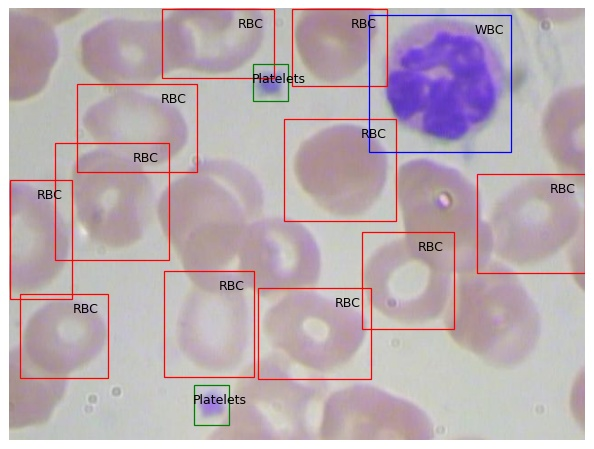
\includegraphics[width=0.40\textwidth]{img/rbc.jpg}
	\legend{Fonte: \citeonline{datasetBCCD}}
	\label{fig:rbc}
\end{figure}

A Figura \ref{fig:rbc} faz parte de um \emph{dataset}\footnote[1]{Um dataset é um grande conjunto de dados coletados.} específico de classificação de células sanguíneas, classificando em \emph{RBC (Red Blood Cells)} para glóbulos vermelhos, \emph{WBC (White Blood Cells)} para glóbulos brancos e \emph{Platelets} para plaquetas.
 
\subsubsection{Glóbulos Brancos}
Os glóbulos brancos, também conhecidos como \emph{White Blood Cells (WBC)}, são as células brancas do sangue, sendo responsáveis pela defesa do organismo contra as principais ameaças do corpo humano presentes no sistema sanguíneo. Através da fagocitose, que é um processo de englobamento de partículas sólidas pelas células, são realizadas ações de defesa contra a invasão de fragmentos estranhos. Os glóbulos brancos são criados na medula óssea e estão presentes em todo o sangue, também em grande quantidade \cite{manualHematologia}.

Algumas células brancas podem ser encontradas na sua forma imatura, que ocorre quando o leucócito ainda não teve uma função definida pelo processo de maturação (promielócitos, mielócitos, metamielócitos). A maturação quando ocorre de forma adequada origina os seguintes tipos de leucócitos, cada qual com sua importância para o sistema de defesa do organismo \cite{manualHematologia}:

\begin{itemize}
	\item \textbf{Neutrófilos}: células brancas mais abundantes, capazes de entrar nos tecidos, onde conseguem realizar a defesa do organismo, fagocitando partículas estranhas. Essas células são conhecidas como neutrófilos segmentados, pois existe uma célula percursora, que é o bastão, ou também chamado de neutrófilos bastonetes, que possuem essa nomenclatura pois seu núcleo não está amadurecido, ou seja ainda são jovens, e geralmente são identificados quando há infecções em fase aguda. 
	\item \textbf{Eosinófilos}: células brancas responsáveis na defesa contra parasitas, geralmente estão presentes em grande quantidade no sangue durante reações alérgicas e infestações parasitárias.
	\item \textbf{Basófilos}: células brancas atuantes em respostas alérgicas e na coagulação do sangue. São capazes de liberar histamina, contribuindo para respostas alérgicas ao dilatar e permeabilizar os vasos sanguíneos e também liberam heparina que é capaz de prevenir a coagulação do sangue.
	\item \textbf{Monócitos}: células brancas capazes de entrar no tecido conjuntivo frouxo, onde conseguem se desenvolver em grandes células, com grande efeito fagocítico denominadas macrófagos, de forma a ingerir partículas estranhas ao organismo.
	\item \textbf{Linfócitos}: segundo tipo de célula branca mais abundante, são responsáveis e de extrema importância nas respostas imunes específicas do corpo humano, inclusive na produção de anticorpos.
\end{itemize}

Percebe-se também na Figura \ref{fig:wbc}, a presença dos glóbulos brancos entre os vermelhos, porém em menor quantidade.

\begin{figure}[!htb]
	\centering
	\caption{Glóbulos Brancos (WBC)}
	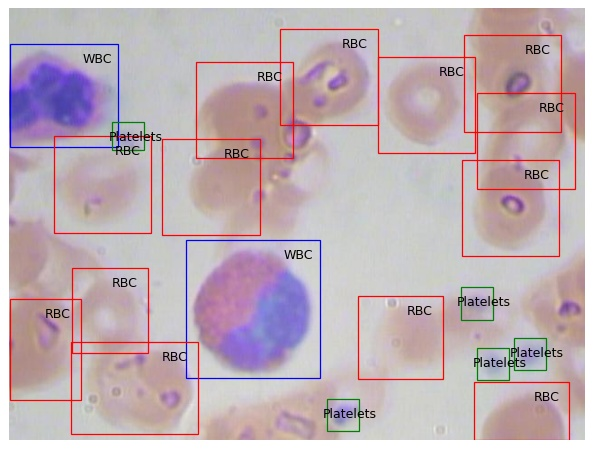
\includegraphics[width=0.40\textwidth]{img/wbc.jpg}
	\legend{Fonte: \citeonline{datasetBCCD}}
	\label{fig:wbc}
\end{figure}

Como visto na Figura \ref{fig:wbc}, embora existam várias classificações de glóbulos brancos, no \emph{dataset} onde foi coletada, não era objetivo de estudo realizar essa análise específica de cada célula.

\subsubsection{Plaquetas}
As plaquetas, também conhecidas e citadas como \emph{Platelets}, são os menores componentes do sangue e possuem grande responsabilidade na hemostasia, que é uma resposta fisiológica para a prevenção e interrupção de sangramentos e hemorragias, ou seja, elas atuam na manutenção dos vasos sanguíneos. As plaquetas são fragmentos do citoplasma de megacariócitos, ou seja, elas são produzidas na medula óssea como parte dessas células especializadas que irão se dividir posteriormente e gerar um grande número de plaquetas. Aproximadamente, para cada 1 megacariócito, pode-se produzir cerca de 4000 plaquetas \cite{abcOfCbc}.

Por serem fragmentos de uma célula, as plaquetas não possuem núcleo e são muito pequenas, com cerca de 1–3 µm\footnote[1]{1 micrômetro (µm) é equivalente à 0,001 milímetro.} de diâmetro, com a coloração azul-acinzentado. A vida útil das plaquetas dura em média de 9 a 12 dias, e elas são removidas pelo baço quando estão velhas ou danificadas \cite{abcOfCbc}.

Percebe-se também através da Figura \ref{fig:plaquetas}, a presença do último elemento visível abordado por este trabalho no \emph{dataset} utilizado como base. Nela é possível visualizar múltiplas plaquetas agrupadas em um dos cantos, além de outras no meio dos demais elementos do sangue.

\begin{figure}[!htb]
	\centering
	\caption{Plaquetas (Platelets)}
	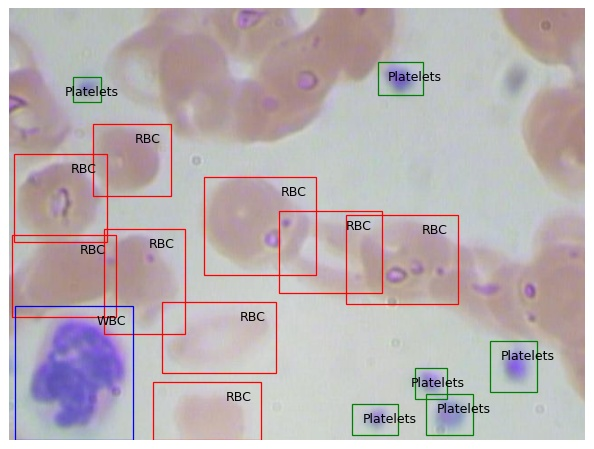
\includegraphics[width=0.40\textwidth]{img/plt.jpg}
	\legend{Fonte: \citeonline{datasetBCCD}}
	\label{fig:plaquetas}
\end{figure}

\subsection{Hemograma}
Um hemograma, também conhecido e citado como \emph{Complete Blood Count (CBC)}, é um exame bastante comum e muito utilizado, onde se realiza uma análise de sangue que envolve a contagem das diferentes células sanguíneas. A partir dos números obtidos através dessa contagem e com a comparação desse valor com as faixas de normalidade, é possível chegar a diversas conclusões sobre a saúde do paciente e até mesmo já identificar alguma doença ou problema \cite{manualHematologia, abcOfCbc}.

Um hemograma é geralmente realizado em duas principais etapas, sendo a primeira relacionada ao eritrograma que se refere à análise das células vermelhas, de forma a revelar até mesmo alguns tipos essenciais de alterações patológicas do sistema eritropoético, sendo o sistema responsável pela produção do material vermelho do sangue, como aumento na produção de glóbulos vermelhos e anemias. A segunda parte está relacionada com o leucograma, que corresponde à contagem global e específica dos leucócitos, a parte branca do sangue \cite{manualHematologia, abcOfCbc}.

\subsubsection{Eritrograma}
O objetivo do eritrograma ao realizar a análise da parte vermelha do sangue, é analisar alguns atributos-chave. Primeiramente é realizada a contagem geral dos eritrócitos adotando uma escala de milhões/mm³. A hemoglobina também é calculada e registrada em uma escala de g/dl \cite{interpretacaoHemograma, manualHematologia}.

Depois dessa principal contagem são calculados alguns índices, que apresenta o primeiro deles o cálculo do volume corpuscular médio (VCM), sendo o volume médio das hemácias, calculado pelo quociente de um determinado volume de hemácias pelo número de células contidas no mesmo. Outro importante atributo é a hemoglobina corpuscular média (HCM), que semelhante ao VCM, apresenta o conteúdo médio da hemoglobina, calculado pelo quociente de conteúdo de hemoglobina em um determinado volume de hemácias pelo número de células contidas no mesmo volume \cite{interpretacaoHemograma, manualHematologia}.

Também temos outro índice que é a concentração de hemoglobina corpuscular média (CHCM), sendo a percentagem da hemoglobina em uma amostra de 100ml de hemácias. Por fim temos, a amplitude de distribuição dos glóbulos vermelhos, que em inglês significa \emph{Red Cell Distribution Width (RDW)}, que será responsável por avaliar a variação de tamanho entre as hemácias \cite{interpretacaoHemograma, manualHematologia}.

É possível visualizar a forma que esses índices do eritrograma estão presentes e são abordados em um hemograma real através da Figura \ref{fig:eritrograma}, assim como os seus respectivos valores de referência.

\begin{figure}[!htb]
	\centering
	\caption{Exemplo de Eritrograma e seus Atributos}
	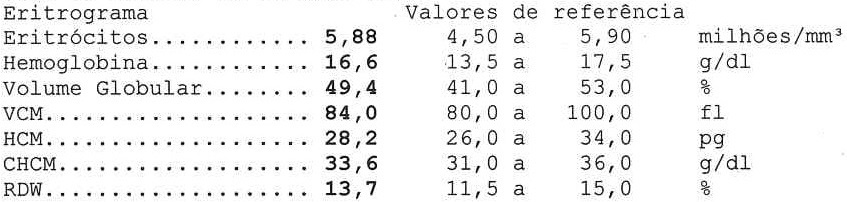
\includegraphics[width=0.80\textwidth]{img/eritrograma.jpg}
	\legend{Fonte: Elaborada pelo autor.}
	\label{fig:eritrograma}
\end{figure}
 
\subsubsection{Leucograma}
O objetivo do leucograma ao realizar a análise da parte branca do sangue, assim como no eritrograma, é analisar alguns atributos-chave, porém, diferente do processo anterior, essa etapa tem um foco muito maior na classificação e contagem de diferentes células brancas.

Primeiramente é feita uma contagem geral de leucócitos em mm³. Depois é realizada a contagem de forma a classificar cada tipo de leucócito presente, com neutrófilos, eosinófilos, basófilos, linfócitos, monócitos e também os granulócitos imaturos (promielócitos, mielócitos, metamielócitos). Por fim, também é calculado o número presente de plaquetas no sangue em mm³ \cite{interpretacaoHemograma, manualHematologia}.

É possível visualizar a maneira que os índices e classificações são abordados em um hemograma real através da Figura \ref{fig:leucograma}, assim como os seus respectivos valores de referência.

\begin{figure}[!htb]
	\centering
	\caption{Exemplo de Leucograma e seus Atributos}
	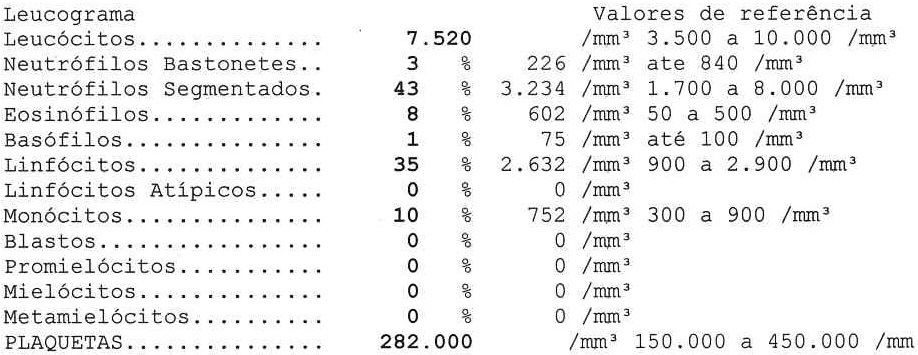
\includegraphics[width=0.80\textwidth]{img/leucograma.jpg}
	\legend{Fonte: Elaborada pelo autor.}
	\label{fig:leucograma}
\end{figure}

\section{Inteligência Artificial: \emph{Machine Learning e Deep Learning}}
\label{sec:conceito2}
A abordagem de \emph{Deep Learning}, que é objeto de estudo desse trabalho é uma das subáreas de \emph{Machine Learning}, que, por sua vez, é subárea de Inteligência Artificial, portanto antes de abordar cada um desses conceitos, quais suas diferenças e aplicações, se faz necessário introduzir o conceito de Inteligência Artificial.

A Inteligência Artificial é uma abordagem para a resolução de problemas de diversas naturezas de forma automatizada, ou seja, é uma maneira de se resolver problemas sem a necessidade de um humano ou usuário específico para esse trabalho. Essa área está recebendo muita atenção atualmente, buscando, cada vez mais, novas maneiras de automatizar tarefas do cotidiano. Essa abordagem está presente em diversos segmentos da indústria e atualmente também vem crescendo o uso nas residências para as mais diversas finalidades \cite{inteligenciaArtificial}.

O intuito dessa área é buscar formas de ensinar máquinas e computadores a serem capazes de ter uma inteligência cada vez mais semelhante aos seres humanos. Isso ocorre geralmente através do reconhecimento de padrões através de diversas técnicas, que permitem que os computadores sejam ensinados a analisar e interpretar dados, de forma semelhante ao que acontece para o aprendizado de seres humanos. Porém, diferente de nós, as máquinas geralmente precisam de um volume massivo de dados para que sejam capazes de aprender algo básico \cite{IAAprendizadoMaquina}.

\subsection{Machine Learning}

A resolução de problemas através de ferramentas da computação é bastante comum e para isso se faz uso de algoritmos programados para finalidades específicas, porém não é em todos os problemas que se pode aplicar essa abordagem tradicional, porque nem sempre se sabe um caminho único de etapas a serem seguidas para chegar a uma resolução. Nesses casos, quando se sabe a entrada de dados e o resultado desejado, mas não os meios para se chegar nesse resultado, é possível utilizar um modelo de \emph{Machine Learning} para realizar a predição. É possível pensar da seguinte forma, na abordagem de algoritmos tradicionais de programação, possuímos os parâmetros necessários e conhecemos o método para assim chegar ao resultado, mas na aplicação de \emph{Machine Learning}, conhecemos os parâmetros e o resultado, porém o método será aprendido e apresentado pela própria máquina \cite{machineLearning}.

É possível fazer uma analogia entre um modelo de \emph{Machine Learning} e uma criança que aprende algo novo, onde todo modelo passa por três principais etapas: o pré-processamento dos dados, a fase de treinamento, e por fim o teste. Na fase de pré-processamento, os dados são analisados e adaptados para um melhor entendimento do modelo, retirando informações inúteis, alterando o formato para um mais adequado, entre outras práticas \cite{machineLearningPython}.

Logo após, o modelo de \emph{Machine Learning} deve ser treinado conforme o método desejado, antes de realizar a predição de qualquer valor ou resultado, onde o responsável pelo treinamento deverá fornecer um grande volume de dados, assim como os resultados esperados em cada um deles, além dos parâmetros e configurações necessárias para o treinamento. Dessa forma o modelo aprende a entender e interpretar os dados, tornando-se ser capaz de reproduzir esse método para prever o resultado de futuros dados \cite{machineLearningPython}.

Por fim, após o treinamento do modelo como um todo ocorre a fase de teste. Nesta fase, o modelo será testado e avaliado com base em algumas técnicas para medir o seu desempenho, calculando métricas como a acurácia, a precisão e a revocação. A acurácia indicará uma performance geral, ou seja, quantas classes o modelo classificou corretamente. A precisão dirá, dentre as classificações que o modelo classificou como positivo, quantas estão corretas. A revocação, também citada como \emph{recall}, apontará dentre todas as classificações que possuem positivo como valor esperado, quantas estão corretas. Além dessas métricas, também existe o F1-Score que realiza uma média harmônica entre precisão e \emph{recall} \cite{machineLearningTensorFlow}.

Para uma melhor visualização, e para realizar o cálculo das métricas citadas anteriormente, se utiliza uma matriz de confusão, que descreve o número de acertos e erros relacionados com os verdadeiros ou falsos positivos e os verdadeiros ou falsos negativos observa-se na Figura \ref{fig:confusionMatrix} \cite{machineLearningTensorFlow}.

\begin{figure}[!htb]
	\centering
	\caption{Matriz de Confusão}
	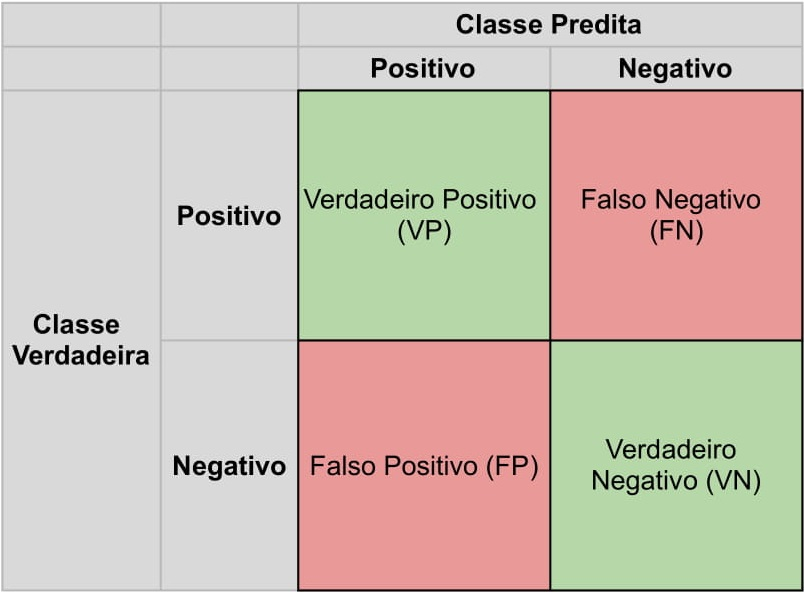
\includegraphics[width=0.50\textwidth]{img/confusionMatrix.jpg}
	\legend{Fonte: Elaborada pelo autor.}
	\label{fig:confusionMatrix}
\end{figure}

\subsubsection{Algoritmos Tradicionais}

Existem várias abordagens de \emph{Machine Learning}, que são divididas em duas metodologias diferentes: supervisionados ou não-supervisionados. No aprendizado supervisionado, sabe-se o resultado correto, ou seja, onde o modelo deverá chegar a partir dos dados obtidos, porém no aprendizado não-supervisionado, o modelo terá que lidar com dados não estruturados e sem um resultado claro \cite{machineLearningPython}.

Dentro do aprendizado supervisionado, encontra-se duas abordagens mais utilizadas, a regressão e a classificação. Os modelos de regressão serão responsáveis pela predição de valores reais, enquanto que os modelos de classificação serão responsáveis pela rotulação dos dados em determinadas classes \cite{machineLearningPython}.

Quando se trabalha com regressão de dados, é possível citar alguns exemplos de abordagens mais utilizadas \cite{machineLearningTensorFlow}.
\begin{itemize}
	\item \textbf{Linear Regression:} método mais clássico e simples para abordar regressão, onde é traçado uma reta através dos dados e então realizado a predição com base nessa reta. Possui variações como na \emph{Multiple Linear Regression} onde são usadas mais variáveis e também na \emph{Polynomial Linear Regression} onde a reta se tornará uma curva, utilizando variáveis com exponenciação, tornando o resultado mais assertivo.
	\item \textbf{Decision Tree:} árvore de decisão é uma técnica utilizada para prever valores através de critérios aprendidos pelo modelo. Esses critérios serão aprendidos através da divisão dos dados conhecidos em grupos semelhantes de forma a encontrar padrões em cada um dos grupos de dados.
	\item \textbf{Random Forest:} floresta aleatória é uma técnica utilizada de forma a combinar o poder de processamento de várias árvores de decisão diferentes, de forma a ter um trabalho mais minucioso e geralmente chegar em um resultado mais preciso.
\end{itemize}

Quando se trabalha com classificação de dados, é possível citar alguns exemplos de algoritmos mais utilizados \cite{machineLearningPython}.
\begin{itemize}
	\item \textbf{K-Nearest Neighbors (KNN):} o KNN é uma abordagem de um algoritmo que realizará a classificação com base na comparação de um dado com dados semelhantes a ele. É considerado uma abordagem \emph{lazy}, ou seja, preguiçosa, pois não apresenta um modelo inteligente, apenas armazena os dados e realiza comparações.
	\item \textbf{Decision Tree Classifier:} assim como na regressão, árvore de decisão é uma técnica utilizada para predizer classes para dados específicos a partir de uma série de critérios aprendidos pelo modelo. Esses critérios serão aprendidos através da divisão dos dados conhecidos em grupos semelhantes de forma a encontrar padrões que nesse caso seriam as classes necessárias para a interpretação em cada um dos grupos divididos de dados.
	\item \textbf{Random Forest Classifier:} assim como na regressão, floresta aleatória é uma técnica utilizada de forma a combinar o poder de processamento de várias árvores de decisão voltadas à classificação, buscando ter um trabalho mais minucioso e geralmente chegar em um resultado mais preciso.
\end{itemize}

Além desses algoritmos, é importante ressaltar uma abordagem diferente da convencional que são as redes neurais, que podem ser utilizadas tanto para regressão quanto para classificação. Esse tipo de abordagem se difere dos algoritmos tradicionais e será objeto de estudo desse trabalho.

\subsubsection{Redes Neurais}
\label{sec:redesneurais}

As redes neurais buscam uma abordagem bastante parecida com o cérebro humano, pois utilizam uma estrutura composta de \emph{perceptrons}, que são uma versão computadorizada de algo parecido com um neurônio humano. O \emph{perceptron} é capaz de receber \emph{inputs} (os dados de entrada) e produzir uma saída. O desempenho do uso de \emph{perceptrons} pode ser melhorado ao utilizar vários em conjunto formando uma rede, assim unindo o poder de processamento de cada um deles e chegando a um resultado mais assertivo em menor tempo. Para essa estrutura se dá o nome de rede neural artificial ou como é conhecida, \emph{Artificial Neural Network} (ANN) \cite{deepLearning, deepLearningTensorFlow}.

A Figura \ref{fig:perceptron} apresenta toda a estrutura de um \emph{perceptron}, onde o x representa a informação repassada, o w representa os pesos de cada informação, a letra $\Sigma$ o somatório, o f a função de ativação e por fim o y representa a saída.

\begin{figure}[!htb]
	\centering
	\caption{\emph{Perceptron}}
	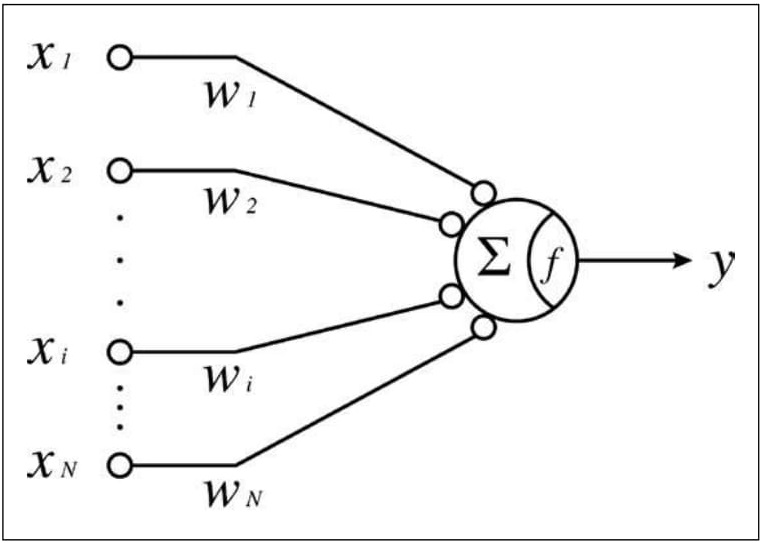
\includegraphics[width=0.50\textwidth]{img/perceptron.jpg}
	\legend{Fonte: \citeonline{deepLearning}}
	\label{fig:perceptron}
\end{figure}

Uma \emph{Artificial Neural Network} é uma estrutura formada por diversos neurônios, conhecidos como \emph{perceptrons}, organizados de forma a imitar o processamento de um cérebro humano. Sua estrutura é definida em diversas camadas, geralmente adotando uma camada de entrada, outra de saída e camadas intermediárias chamadas de ocultas que serão responsáveis pelo processamento na totalidade, onde cada uma delas pode conter um número variável de \emph{perceptrons} \cite{deepLearningTensorFlow}. Pode-se visualizar esta estrutura na Figura \ref{fig:neuralNetwork}, com a presença da camada de entrada, as camadas escondidas e por fim a camada de saída.

\begin{figure}[!htb]
	\centering
	\caption{Artificial Neural Network}
	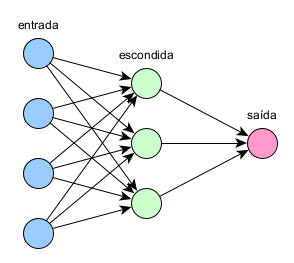
\includegraphics[width=0.40\textwidth]{img/neuralNetwork.png}
	\legend{Fonte: Elaborada pelo autor.}
	\label{fig:neuralNetwork}
\end{figure}

É importante ressaltar que além das informações repassadas de um \emph{perceptron} para o outro, existe outro fator importantíssimo para o seu funcionamento, sendo os pesos adotados. Os pesos são valores definidos para cada informação recebida pelo \emph{perceptron} e pode-se pensar no seu uso como um critério de prioridade entre uma informação e outra, que serão ajustados para alcançar o resultado desejado \cite{deepLearningTensorFlow}.

Dessa forma, uma ANN poderá aprender a realizar diversos tipos de tarefas, como classificação, por exemplo, através do uso de um algoritmo de \emph{backpropagation} que significa propagação regressiva, responsável por gerir a taxa de aprendizado do modelo, seguindo alguns passos \cite{deepLearningTensorFlow}.

Primeiramente, o algoritmo inicia a rede artificial com pesos aleatórios, entrando em modo de treino para realizar o aprendizado. Durante o treinamento, o algoritmo é capaz de realizar predições de resultados que serão comparados com os valores corretos, para saber se está obtendo sucesso ou não. O algoritmo de \emph{backpropagation} então calcula a diferença do resultado obtido com o real, e essa informação do erro é repassada para todas as camadas anteriores de forma a realizar um ajuste nos pesos e minimizar o erro \cite{deepLearningTensorFlow}.

Todo esse processo é realizado muitas vezes durante o treinamento, e só encerra quando os ajustes levam ao aumento do erro novamente, indicando que os pesos foram ajustados até o limite. Essa etapa de otimização dos pesos utilizados pela rede é muito importante, sendo essencial para o funcionamento da rede neural, pois através dela que é possível para o modelo aprender com os seus erros \cite{deepLearningTensorFlow}.

\subsection{Deep Learning}
Existem alguns casos que o \emph{Machine Learning} não é suficiente para o aprendizado a partir dos dados, pois o aprendizado acontece através de reconhecimento de padrões com base nos dados que não podem ser utilizados de qualquer forma, devem ser preparados e adaptados para cada modelo, ou seja, a máquina não é capaz de aprender por conta própria, pois precisa sempre de intervenção humana para o processamento dos dados. Logo, é preciso uma abordagem muito mais parecida com a forma de pensar dos seres humanos, como o \emph{Deep Learning} \cite{deepLearningPython, deepLearningTensorFlow}.

O \emph{Deep Learning} busca formas de aprofundar o conceito das redes neurais abordado na seção \ref{sec:redesneurais}, utilizando \emph{Deep Neural Networks (DNNs)}. As \emph{Deep Neural Networks (DNNs)}, ou Redes Neurais Profundas, são uma arquitetura de rede neural orientada ao \emph{Deep Learning}, ou seja, são muito mais complexas em seus modelos, com um número maior de neurônios, camadas ocultas em configurações mais complexas e conexões específicas entre os neurônios \cite{deepLearningTensorFlow}.

Com as possibilidades que as redes neurais profundas trouxeram, surgiram algumas variantes interessantes e focadas em um nicho específico, buscando se assemelhar ainda mais a natureza humana para realizar tarefas e criar inteligência. Algumas dessas variantes se aplicam a processamento de linguagem natural, como é o caso das RNNs abordadas na seção \ref{sec:rnn}, ou também abordam o reconhecimento e interpretação de imagens como é o caso das CNNs abordadas na seção \ref{sec:cnn} e é assunto de interesse para a continuidade deste trabalho.

\subsubsection{\emph{Recurrent Neural Networks (RNNs)}}
\label{sec:rnn}
As \emph{Recurrent Neural Networks}, ou Redes Neurais Recorrentes, são uma arquitetura de rede neural desenvolvida para a interpretação de dados temporais em sequência, ou seja, podem realizar predições de variáveis em relação ao tempo. Sua estrutura é desenvolvida para permitir conexões de feedback das informações repassadas, ou seja, possui \emph{loops} que permitem que as informações persistam, como se a rede fosse executada várias vezes. As RNNs são desenvolvidas para utilizar informações que possuem uma sequência fixa, como é o caso de informações que são atualizadas em decorrência do tempo \cite{deepLearningTensorFlow}.

\subsubsection{\emph{Convolutional Neural Networks (CNNs)}}
\label{sec:cnn}
As \emph{Convolutional Neural Networks}, ou Redes Neurais Convolucionais, são uma arquitetura de rede neural desenvolvida especificamente para o reconhecimento de imagens, com a capacidade de interpretar imagens dividindo-as em partes importantes. Essa rede trabalha inicialmente com 3 informações base, interpretando imagens como matrizes de 3 dimensões, sendo a altura, a largura e a cor \cite{deepLearningTensorFlow}.

As DNNs tradicionais funcionam bem para imagens pequenas, porém com um grande volume de dados, que nesse caso será cada pixel da imagem, o modelo teria muita dificuldade para aprender, logo nasceu a necessidade das CNNs. Para resolver esse problema, as CNNs foram desenvolvidas para usar camadas parcialmente conectadas e com grande reutilização dos pesos, dessa forma tem muito menos parâmetros à interpretar e passar adiante e consequentemente são mais rápidas para treinar, tendo menor risco de sobre-ajuste e necessitando de um volume menor de dados de treinamento \cite{deepLearningTensorFlow}.

Essa eficiência se deve também ao fato de que uma CNN, quando aprender a interpretar algum recurso ou elemento específico na imagem, se torna capaz de identificar aquele elemento em qualquer lugar da imagem, diferentemente das DNNs que só aprendem a reconhecer um recurso em um local fixo. Isso mostra a capacidade das CNNs de serem mais generalistas em comparação com as DNNs \cite{deepLearningTensorFlow}.

Esse recurso pode ser encontrado dentro da camada convolucional, que está presente no início do processo e pode ser observada na Figura \ref{fig:cnn}. 

\begin{figure}[!htb]
	\centering
	\caption{Convolutional Neural Network}
	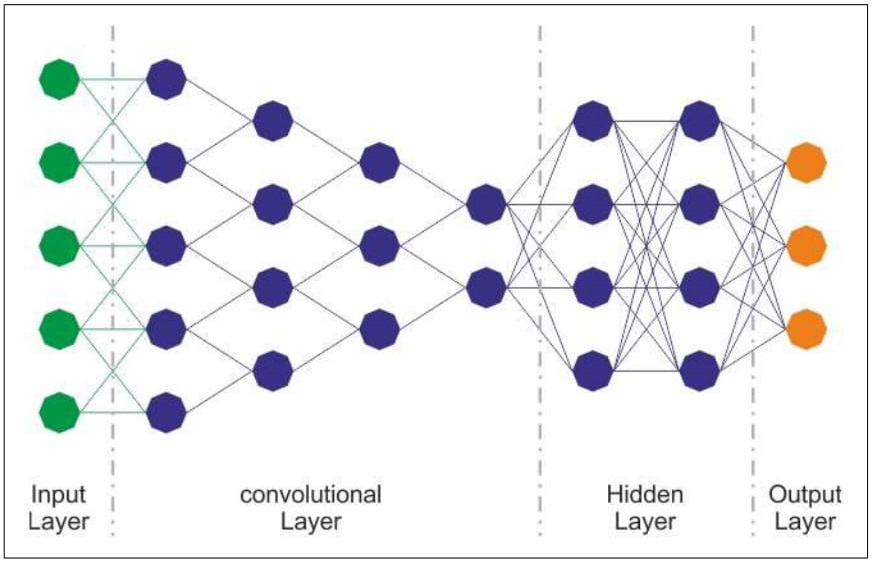
\includegraphics[width=0.60\textwidth]{img/cnn.jpg}
	\legend{Fonte: \citeonline{deepLearningTensorFlow}}
	\label{fig:cnn}
\end{figure}

\subsubsection{Bibliotecas e Recursos}
Para se trabalhar com \emph{Deep Learning} e suas principais arquiteturas e recursos, existem algumas bibliotecas disponíveis no mercado gratuitamente, as quais tendem a facilitar e orientar esse trabalho. Dessa forma, pode-se encontrar o Tensorflow e o Keras, sendo duas bibliotecas desenvolvidas em Python e C++, com a possibilidade de se trabalhar em conjunto e muito utilizadas pela comunidade de \emph{Deep Learning} em geral \cite{deepLearningTensorFlow}.

O Tensorflow é uma plataforma completa de código aberto para \emph{Machine Learning}, a qual considera uma grande variedade de tarefas com um foco nas redes neurais, porém suas funcionalidades também se estendem ao \emph{Deep Learning}. As APIs disponibilizadas do Tensorflow utilizam como base o próprio Keras para definir e treinar as redes neurais. Desenvolvido pelo Google desde 2011, em 2018 a equipe decidiu integrar o Keras na biblioteca principal do Tensorflow \cite{websiteTensorFlow}.

O Keras foi desenvolvido para permitir uma experimentação e prototipação rápida, com um principal foco nas redes neurais profundas. Promete ser fácil de utilizar, modular e ainda ser extensível. Possui vários recursos próprios, como a utilização de camadas, funções de perda, funções de ativação, entre outros. Além do foco em redes neurais profundas, possui módulos voltados a redes neurais convolucionais e recorrentes \cite{websiteKeras}.

O conjunto dessas duas bibliotecas para o trabalho com \emph{Machine Learning} e \emph{Deep Learning}, torna-se uma ferramenta extramente útil para este fim, possibilitando trabalhar com vários tipos de dados, como número, texto, áudio e também imagens.

Através da documentação do Tensorflow, é possível encontrar informações para desenvolver uma rede neural convolucional, por exemplo, onde existe toda a parte teórica e também a demonstração de um exemplo prático voltado a esse fim. Também é possível através dessa biblioteca e da sua documentação estar realizando a classificação de imagens com base em um \emph{dataset} de imagens \cite{websiteTensorFlow}.

\chapter{Estado da Arte da Área Pesquisada}
\label{chap:mapeamento}

O processo de pesquisa e seleção dos trabalhos relacionados, foi realizado com base em um mapeamento sistemático sobre as pesquisas com propostas para agilizar a identificação e interpretação de hemogramas. Este mapeamento resultou na identificação e seleção dos principais trabalhos de pesquisa no tema deste Projeto de Trabalho de Conclusão de Curso. Outro objetivo deste mapeamento sistemático foi verificar os métodos utilizados para a aplicação de \emph{Deep Learning} em imagens de sangue em placas de Petri de maneira que possam ser obtidas informações para a geração automatizada de hemogramas.

\section{Mapeamento Sistemático da Literatura}

O mapeamento sistemático da literatura foi realizado com base na busca e levantamento de artigos, utilizando uma string de busca\footnote[1]{Uma string de busca é um conjunto de palavras-chave organizadas para auxiliar na pesquisa.} nas principais bibliotecas e repositórios de artigos. Esses artigos foram analisados e selecionados conforme a sua área de pesquisa e a sua temática, para inclusão nesse estudo. Para gerenciar o mapeamento sistemático foi utilizado a ferramenta Parsifal\footnote[2]{https://parsif.al/}, a qual auxilia na definição da string de busca, e permite salvar os artigos necessários e realizar a seleção.

As questões de pesquisas levantadas para isso foram, ``Como os algoritmos de \emph{Deep Learning} podem ser utilizados para a interpretação de exames?'' e ``Como realizar o tratamento de imagens para reconhecimento por modelos de \emph{Deep Learning}?''. A partir dessas questões foram extraídas palavras e termos para o direcionamento da pesquisa. É possível visualizar estas palavras com seus sinônimos na Tabela 1.

\begin{table}[!htb]
	\centering
	\caption{Palavras-Chave e Sinônimos}
	\label{tbl:palavrasChave}
	\begin{tabular}{|c|c|}
		\hline
		\textbf{Palavra-Chave} & \textbf{Sinônimos}                                        \\ \hline
		Blood Analysis         & Blood Sample                                               \\ \hline
		Classification         & Interpretation, Recognition                                \\ \hline
		Deep Learning          & Artificial Intelligence, Computer Vision, Machine Learning \\ \hline
	\end{tabular}
	\vspace{6pt}
	\legend{Fonte: Elaborada pelo autor.}
\end{table}

Na Tabela 2, são listadas as bases de dados onde os artigos foram coletados, a quantidade de cada um deles e a string de busca utilizada na seleção. A mesma string de busca foi utilizada nas três bases de dados, e os artigos encontrados foram dos últimos 5 anos (2016-2021).

\begin{table}[!htb]
	\centering
	\caption{Bases de Dados e Número de Artigos Selecionados}
	\label{tbl:basesDeDados}
	\begin{tabular}{|c|c|c|}
		\hline
		\textbf{Base de Dados}                & \textbf{Artigos}     & \textbf{String de Busca}                                                                                     \\ \hline
		\multirow{2}{*}{ACM Digital Library}  & \multirow{2}{*}{37}  & \multirow{6}{*}{\begin{tabular}[c]{@{}c@{}}(``classification'' OR ``interpretation'' OR ``recognition'') AND \\  (``deep learning'' OR ``artificial intelligence'' \\ OR ``computer vision'' OR ``machine learning'') AND\\  (``blood analysis'' OR ``blood sample'')\end{tabular}} \\
		                                      &                      &                                                                                                              \\ \cline{1-2}
		\multirow{2}{*}{IEEE Digital Library} & \multirow{2}{*}{13}  &                                                                                                              \\
		                                      &                      &                                                                                                              \\ \cline{1-2}
		\multirow{2}{*}{Scopus}               & \multirow{2}{*}{114} &                                                                                                              \\
		                                      &                      &                                                                                                              \\ \hline
	\end{tabular}
	\vspace{6pt}
	\legend{Fonte: Elaborada pelo autor.}
\end{table}

\subsection{Critérios de Exclusão}

Os artigos coletados na pesquisa através da string de busca, passaram por critérios de exclusão por não se adequarem a esta pesquisa, esses critérios podem ser observados na Tabela 3. 

\begin{table}[!htb]
	\centering
	\caption{Critérios de Exclusão}
	\label{tbl:exclusao}
	\begin{tabular}{|c|c|}
		\hline
		\textbf{Critério de Exclusão}                    & \textbf{Nº de Artigos Recusados} \\ \hline
		O estudo não faz parte da área de pesquisa       & 101                               \\ \hline
		O estudo apresenta resultados fora da computação & 29                                \\ \hline
		O estudo não é um estudo primário               & 6                                 \\ \hline
		O estudo é duplicado                              & 16                                \\ \hline
	\end{tabular}
	\vspace{6pt}
	\legend{Fonte: Elaborada pelo autor.}
\end{table}

A seleção iniciou com 164 artigos no total das três bases de dados pesquisadas. Com a aplicação dos critérios de exclusão, observa-se um resultante de apenas 12 artigos. Isso ocorreu, pois, 101 artigos foram eliminados no critério ``O estudo não faz parte da área de pesquisa'', que significa que esses artigos tinham alguma relação, porém eram voltados a outras áreas. Outros 29 artigos foram eliminados no critério ``O estudo apresenta resultados fora da computação'', que significa serem da área de pesquisa, porém com resultados e métodos sem conexão com a computação. Foram também encontrados 6 artigos, que foram eliminados no critério ``O estudo não é um estudo primário'', o que indica que o artigo pode ser uma revisão sistemática da literatura ou semelhante. Por fim, foram eliminados outros 16 artigos por serem duplicados.

\subsection{Critérios de Inclusão}

Os seguintes critérios de inclusão foram definidos:
\begin{itemize}
	\item Nova tecnologia para análise de hemogramas;
	\item Processo, método ou técnica para contagem de células sanguíneas;
	\item Sistema para elaboração de hemogramas utilizando Deep Learning;
\end{itemize}

Na Tabela 4, é possível visualizar todos os 12 artigos selecionados com base nos critérios de inclusão, uma vez que todos eles se enquadram em pelo menos um deles.

\begin{table}[!htb]
	\centering
	\caption{Artigos Selecionados}
	\label{tbl:mapeamento}
	\begin{tabular}{|c|l|l|}
		\hline
		\textbf{ID} & \multicolumn{1}{c|}{\textbf{Título do Artigo}} & \multicolumn{1}{c|}{\textbf{Autores}}                     \\ \hline
		A1          & \begin{tabular}[c]{@{}l@{}}Analyzing microscopic images of           \\ peripheral blood smear \\ using deep learning\end{tabular} & \begin{tabular}[c]{@{}l@{}}Mundhra, D. and Cheluvaraju, B. \\ and Rampure, J. and Rai Dastidar, T.\end{tabular} \\ \hline
		A2          & \begin{tabular}[c]{@{}l@{}}Automatic detection and classification    \\ of leukocytes using \\ convolutional neural networks\end{tabular} & \begin{tabular}[c]{@{}l@{}}Zhao, J. and Zhang, M. \\ and Zhou, Z. and Chu, J. and Cao, F.\end{tabular} \\ \hline
		A3          & \begin{tabular}[c]{@{}l@{}}Automatic white blood cell classification \\ using pre-trained deep learning models: \\ ResNet and Inception\end{tabular} & \begin{tabular}[c]{@{}l@{}}Habibzadeh, M. and Jannesari, M. \\ and Rezaei, Z. and Baharvand, H. \\ and Totonchi, M.\end{tabular} \\ \hline
		A4          & \begin{tabular}[c]{@{}l@{}}Classification of Human White             \\ Blood Cells Using Machine Learning \\ for Stain-Free Imaging \\ Flow Cytometry\end{tabular} & \begin{tabular}[c]{@{}l@{}}Lippeveld, M. and Knill, C. and \\ Ladlow, E. and \\ Fuller, A. and Michaelis, L.J. and \\ Saeys, Y. and Filby, A. and Peralta, D.\end{tabular} \\ \hline
		A5          & \begin{tabular}[c]{@{}l@{}}Blood cell classification using the hough \\ transform and \\ convolutional neural networks\end{tabular} & \begin{tabular}[c]{@{}l@{}}Molina-Cabello, M.A. and López-Rubio, E. \\ and Luque-Baena, R.M. and \\ Rodríguez-Espinosa, M.J. and \\ Thurnhofer-Hemsi, K.\end{tabular} \\ \hline
		A6          & \begin{tabular}[c]{@{}l@{}}White Blood Cells Image Classification    \\ Using Deep Learning with \\ Canonical Correlation Analysis\end{tabular} & Patil, A.M. and Patil, M.D. and Birajdar, G.K. \\ \hline
		A7          & \begin{tabular}[c]{@{}l@{}}Image processing and machine learning     \\ in the morphological analysis \\ of blood cells\end{tabular} & \begin{tabular}[c]{@{}l@{}}Rodellar, J. and Alférez, S. and Acevedo, A. \\ and Molina, A. and Merino, A.\end{tabular} \\ \hline
		A8          & \begin{tabular}[c]{@{}l@{}}Improving blood cells classification in   \\ peripheral blood smears using \\ enhanced incremental training\end{tabular} & Al-qudah, R. and Suen, C.Y. \\ \hline
		A9          & \begin{tabular}[c]{@{}l@{}}Corruption-Robust Enhancement of          \\ Deep Neural Networks\\ for Classification of Peripheral \\ Blood Smear Images\end{tabular} & \begin{tabular}[c]{@{}l@{}}Zhang, S. and Ni, Q. and Li, B. and \\ Jiang, S. and \\ Cai, W. and Chen, H. and Luo, L.\end{tabular} \\ \hline
		A10         & \begin{tabular}[c]{@{}l@{}}Convolutional neural network and decision \\ support in medical imaging:\\ Case study of the recognition of \\ blood cell subtypes\end{tabular} & Diouf, D. and Seck, D. and Diop, M. and Ba, A. \\ \hline
		A11         & \begin{tabular}[c]{@{}l@{}}Combining Convolutional Neural Network    \\ With Recursive Neural Network \\ for Blood Cell Image Classification\end{tabular} & \begin{tabular}[c]{@{}l@{}}Liang, G. and Hong, H. and Xie, W. and\\ Zheng, L.\end{tabular} \\ \hline
		A12         & \begin{tabular}[c]{@{}l@{}}Blood diseases detection using            \\ classical machine learning algorithms\end{tabular} & Alsheref, F.K. and Gomaa, W.H. \\ \hline
	\end{tabular}
	\vspace{6pt}
	\legend{Fonte: Elaborada pelo autor.}
\end{table}

Todos os artigos selecionados estão relacionados à recursos para auxiliar na interpretação de exames de sangue utilizando conceitos de \emph{Deep Learning} e \emph{Machine Learning}.

\section{Análise dos trabalhos selecionados}

Por fim, com os artigos selecionados e classificados, foi realizada a extração dos dados desses trabalhos, sendo essa a última etapa desse mapeamento sistemático da literatura. É possível perceber que os algoritmos e abordagens mais utilizados são técnicas de \emph{Deep Learning}, como, por exemplo, o uso de \emph{Convolutional Neural Network (CNN)} (A1, A2, A3, A4, A5, A6, A8, A9, A10, A11) e de \emph{Recurrent Neural Network (RNN)} (A6, A11), sendo abordagens de redes neurais para a classificação das células sanguíneas.

Outros trabalhos utilizam de algoritmos de \emph{Machine Learning} tradicionais para a classificação, como por exemplo, o uso de \emph{Random Forest} ou \emph{Decision Trees}  (A2, A4, A7), sendo estruturas de árvores de decisão. Também foram encontrados estudos recorrendo a \emph{Support Vector Machine (SVM)} (A7) que utilizam vetores de suporte e por fim \emph{K-Means e K-Nearest Neighbors (KNN)} (A12), que faz a classificação considerando os vizinhos mais próximos.

\chapter{Metodologia}
\label{chap:metodologia}
% Quanto à natureza = Aplicada
% Quanto ao estilo de pesquisa = Empírica
% Quanto aos objetivos = Exploratória
% Quanto aos procedimentos metodológicos = Bibliográfica e Experimental

O projeto iniciou com uma pesquisa exploratória da bibliografia para delimitar o escopo e compreender melhor os aspectos que estão sendo aplicados para o domínio de problema abordado por este trabalho. Essa pesquisa exploratória permitiu elaborar um mapeamento sistemático da literatura e também desenvolver a fundamentação teórica a partir disso.

Na sequência deste trabalho serão coletados dos \emph{datasets} de imagens selecionados para a pesquisa. Com base em uma análise aprofundada desse material, serão realizados os devidos tratamentos, de forma a preparar uma base de dados sólida e confiável para o prosseguimento dos trabalhos. Esses \emph{datasets} estão disponíveis na internet de forma aberta e gratuita.

Com o \emph{dataset} devidamente ajustado, será iniciada a preparação do modelo de \emph{Deep Learning}, objetivando definir as camadas que o modelo deverá ter, com base nas imagens contidas no \emph{dataset}. Com o modelo desenvolvido, será iniciada a fase de treinamento, para então realizar o teste do modelo em si. Para que isso seja possível o \emph{dataset} será divido em duas partes, adotando uma proporção de 70\% das imagens para o treino e 30\% para o teste.

Os modelos de \emph{Deep Learning} após esse processo podem ser avaliados em relação ao seu desempenho, verificando métricas importantes do aprendizado como acurácia, sendo a linear ou categórica. Além dessa análise, se pode também preparar uma matriz de confusão para uma melhor visualização do desempenho do modelo. Dependendo do resultado recebido, o modelo poderá passar por modificações e melhorias para um resultado mais assertivo e consequentemente mais confiável.

Por fim, ao atingir o objetivo desejado, os dados dos resultados e da performance do modelo serão registrados e descritos no trabalho de conclusão de curso em forma de monografia. Além disso, será feita uma comparação dessa solução com as demais encontradas por outros modelos documentados na literatura.

\chapter{Resultados}
\label{chap:resultados}


\chapter{Conclusões}
\label{chap:conclusoes}

Este projeto iniciou com o interesse de utilizar as técnicas de \emph{Deep Learning} para auxiliar os profissionais da saúde em seus trabalhos, pois com a automatização que essa técnica oferece, outras tarefas podem ter maior atenção. O hemograma é o exame mais básico, mais essencial e também o mais realizado. Portanto, os estudos subsequentes foram direcionados a estudar quais seriam as melhores abordagens para a automatização dessa tarefa.

Foi possível entender todo o processo de produção de hemograma e também encontrar as formas de associar os conceitos de \emph{Deep Learning} nesse processo. Através do treinamento de um modelo computacional inteligente capaz de reconhecer as diferentes células do sangue, desenvolveu-se a contagem de todas os tipos de célula com grande precisão.

Essa abordagem desenvolvida é de grande utilidade, pois permite tirar conclusões sobre o estado atual da saúde do paciente. A contagem das células brancas, vermelhas e também das plaquetas, permitem avaliar se existe algum desequilíbrio em seus níveis, caso apresente algum fator anormal, outros exames mais aprofundados podem ser realizados para verificar estas questões. Entretanto, não se caracteriza como um hemograma completo, pois devido a limitações do \emph{dataset} utilizado, o trabalho também apresentou limitações, principalmente relacionado a classificação das células brancas, onde a contagem foi geral.

Para estudos futuros, é possível utilizar os conceitos aqui abordados para aplicar estes conhecimentos em um conjunto de dados diferente e mais complexo, ou também voltado para outro fim. Com poucas adaptações é possível continuar a abordagem adotada por este trabalho para contribuir na literatura, calculando a contagem em relação ao volume e posteriormente buscando reproduzir todas as informações presentes em um hemograma.


% ----------------------------------------------------------
% Elementos Pós-Textuais
% ----------------------------------------------------------
\postextual

% ----------------------------------------------------------
% Referências Bibliográficas
% ----------------------------------------------------------
\bibliography{referencias}

%% ----------------------------------------------------------
% Apêndices
% ----------------------------------------------------------
\begin{apendicesenv}
	% Imprime uma página indicando o início dos apêndices
	%\partapendices
	
	\chapter{Meu primeiro apêndice}
	\lipsum[50]
	
\end{apendicesenv}

% ----------------------------------------------------------
% Anexos
% ----------------------------------------------------------
\begin{anexosenv}
	% Imprime uma página indicando o início dos anexos
	%\partanexos
	
	\chapter{Meu primeiro assunto de anexo}
	\lipsum[30]
	
	\chapter{Segundo assunto que pesquisei}
	\lipsum[31]
	
\end{anexosenv} % anexos (se houver)
\end{document}